\documentclass[11pt,a4paper]{article}
\usepackage[a4paper,margin=2.2cm,top=2.2cm,bottom=2.4cm]{geometry}
\usepackage[T1]{fontenc}
\usepackage{lmodern}
\usepackage{amsmath,amssymb,bm}
\usepackage{xcolor,enumitem,titlesec,graphicx,booktabs,fancyvrb,float,caption,longtable,fancyhdr,array}
\usepackage{tikz}\usetikzlibrary{arrows.meta,positioning,calc,decorations.pathreplacing}
\usepackage[hidelinks]{hyperref}
\definecolor{soft}{gray}{0.93}
\definecolor{acc}{HTML}{B00020}
\definecolor{ckf}{HTML}{2A78D6}\definecolor{codo}{HTML}{EB6834}\definecolor{ccam}{HTML}{1BAF7A}
\titleformat{\section}{\large\bfseries}{\thesection\quad}{0pt}{}[\titlerule]
\titlespacing*{\section}{0pt}{14pt}{6pt}
\titleformat{\subsection}{\normalsize\bfseries}{\thesubsection\quad}{0pt}{}
\titlespacing*{\subsection}{0pt}{9pt}{3pt}
\setlength{\parindent}{0pt}
\setlength{\parskip}{5pt}
\setlist{nosep,leftmargin=1.5em,itemsep=3pt}
\pagestyle{fancy}\fancyhf{}
\renewcommand{\headrulewidth}{0pt}\renewcommand{\footrulewidth}{0.4pt}
\lfoot{KFUPM Controls \& Instrumentation}\cfoot{\thepage}\rfoot{Prof. Aamer Iqbal Bhatti}
\emergencystretch=3em
\sloppy
\captionsetup{font=small,labelfont=bf}

% ======================= EDIT HERE: demonstration video link =======================
\newcommand{\videolink}{submitted to the official course channel}
% ====================================================================================

\newcommand{\todo}[1]{\textcolor{acc}{\textbf{[TODO: #1]}}}
\newcommand{\figorti}[3]{\IfFileExists{#1}{\includegraphics[width=#2\linewidth]{#1}}{\colorbox{soft}{\parbox{\dimexpr#2\linewidth-2\fboxsep}{\centering\vspace{1.2cm}\todo{#3}\vspace{1.2cm}}}}}

% numbers: placeholders first, then the files written by the analysis scripts (real robot data only)
% Placeholders shown until scripts/analyze.py writes results.tex from the real trials.
\newcommand{\HaveResults}{0}
\newcommand{\ResN}{\todo{n}}
\newcommand{\ResNexcl}{\todo{excl.}}
\newcommand{\ResStart}{1.50}
\newcommand{\ResStop}{0.50}
\newcommand{\ResMAE}{\todo{MAE}}
\newcommand{\ResRange}{\todo{range}}
\newcommand{\ResMin}{\todo{min}}
\newcommand{\ResMax}{\todo{max}}
\newcommand{\ResBias}{\todo{bias}}
\newcommand{\ResSD}{\todo{SD}}
\newcommand{\ResRMSE}{\todo{RMSE}}
\newcommand{\ResCI}{\todo{CI}}
\newcommand{\ResPt}{\todo{p}}
\newcommand{\ResPsw}{\todo{p}}
\newcommand{\ResOdomMAE}{\todo{odom MAE}}
\newcommand{\ResOdomRange}{\todo{odom range}}
\newcommand{\ResOdomBias}{\todo{odom bias}}
\newcommand{\ResOdomSD}{\todo{odom SD}}
\newcommand{\ResCamMAE}{\todo{camera MAE}}
\newcommand{\ResCamRange}{\todo{camera range}}
\newcommand{\ResCamBias}{\todo{camera bias}}
\newcommand{\ResImprove}{\todo{\%}}
\newcommand{\ResWilOdom}{\todo{p}}
\newcommand{\ResWilCam}{\todo{p}}
\newcommand{\ResStopMean}{\todo{mean}}
\newcommand{\ResStopSD}{\todo{SD}}
\newcommand{\ResStopMin}{\todo{min}}
\newcommand{\ResStopMax}{\todo{max}}
\newcommand{\ResCorrMean}{\todo{corr.}}
\newcommand{\ResCorrMaxAbs}{\todo{corr.}}
\newcommand{\ResHz}{\todo{Hz}}
\newcommand{\ResDetect}{\todo{\%}}
\newcommand{\ResRollout}{\todo{cm}}
\newcommand{\ResSigmaMean}{\todo{mm}}
\newcommand{\ResCover}{\todo{\%}}
\newcommand{\ResLatency}{\todo{s}}
\newcommand{\ResLateral}{\todo{mm}}
\newcommand{\ResLateralMax}{\todo{mm}}
\newcommand{\ResBearingMax}{\todo{deg}}

\newcommand{\HaveCalib}{0}\newcommand{\CalA}{\todo{a}}\newcommand{\CalB}{\todo{b}}\newcommand{\CalCzero}{\todo{c0}}
\newcommand{\CalCone}{\todo{c1}}\newcommand{\CalRMS}{\todo{RMS}}\newcommand{\CalN}{\todo{N}}
\newcommand{\HaveLatency}{0}\newcommand{\LatL}{\todo{L}}\newcommand{\LatRMS}{\todo{mm}}\newcommand{\LatRMSzero}{\todo{mm}}
\newcommand{\LatRuns}{\todo{runs}}
\IfFileExists{results.tex}{% written by scripts/analyze.py - do not edit by hand
\renewcommand{\ResN}{10}
\renewcommand{\ResNexcl}{0}
\renewcommand{\ResStart}{1.50}
\renewcommand{\ResStop}{0.50}
\renewcommand{\ResMAE}{21.0}
\renewcommand{\ResRange}{39.4}
\renewcommand{\ResMin}{+4.5}
\renewcommand{\ResMax}{+43.9}
\renewcommand{\ResBias}{+21.0}
\renewcommand{\ResSD}{14.7}
\renewcommand{\ResRMSE}{25.2}
\renewcommand{\ResCI}{[+10.5, +31.5]}
\renewcommand{\ResPt}{0.001}
\renewcommand{\ResPsw}{0.230}
\renewcommand{\ResOdomMAE}{31.3}
\renewcommand{\ResOdomRange}{101.2}
\renewcommand{\ResOdomBias}{+11.9}
\renewcommand{\ResOdomSD}{35.2}
\renewcommand{\ResCamMAE}{22.3}
\renewcommand{\ResCamRange}{41.0}
\renewcommand{\ResCamBias}{+22.3}
\renewcommand{\ResImprove}{33}
\renewcommand{\ResWilOdom}{0.064}
\renewcommand{\ResWilCam}{0.010}
\renewcommand{\ResStopMean}{0.4718}
\renewcommand{\ResStopSD}{16.0}
\renewcommand{\ResStopMin}{0.4500}
\renewcommand{\ResStopMax}{0.4920}
\renewcommand{\ResCorrMean}{+9.1}
\renewcommand{\ResCorrMaxAbs}{46.3}
\renewcommand{\ResHz}{22.3}
\renewcommand{\ResDetect}{100}
\renewcommand{\ResRollout}{1.0}
\renewcommand{\ResSigmaMean}{1.5}
\renewcommand{\ResCover}{0}
\renewcommand{\ResLatency}{0.015}
\renewcommand{\ResLateral}{3.3}
\renewcommand{\ResLateralMax}{8.8}
\renewcommand{\ResBearingMax}{5.8}
\renewcommand{\HaveResults}{1}
}{}
\IfFileExists{calib.tex}{% written by scripts/fit_calib.py
\renewcommand{\CalA}{0.9724}
\renewcommand{\CalB}{-0.0389}
\renewcommand{\CalCzero}{9.4}
\renewcommand{\CalCone}{4.4}
\renewcommand{\CalRMS}{34.8}
\renewcommand{\CalN}{12}
\renewcommand{\HaveCalib}{1}
}{}
\IfFileExists{latency.tex}{% written by scripts/estimate_latency.py
\renewcommand{\LatL}{0.015}
\renewcommand{\LatRMS}{7.5}
\renewcommand{\LatRMSzero}{7.6}
\renewcommand{\LatRuns}{2}
\renewcommand{\HaveLatency}{1}
}{}
\newcommand{\tabortodo}[2]{\IfFileExists{#1}{\input{#1}}{\todo{#2}}}

\begin{document}

\begin{center}
{\LARGE\bfseries SCE 672: Advanced Robotics}\\[5pt]
{\large\bfseries Project Phase 3: RoboMaster Odometry --- Prediction and Correction of the Distance to a Fixed Tag}
\end{center}
\noindent\textbf{Student:} Ameen Ur Rehman (202527430)\\
\textbf{Instructor:} Prof. Aamer Iqbal Bhatti\\
\textbf{Institution:} King Fahd University of Petroleum \& Minerals\\
\textbf{Code and data:} \url{https://github.com/AmeenUrRehman/RoboMaster-Advanced-Robotics} (folder \texttt{Assignment 3})\\
\textbf{Video:} \videolink
\par\vspace{2pt}\noindent\rule{\linewidth}{0.8pt}

\begin{abstract}\noindent
A DJI RoboMaster EP Core, controlled from Ubuntu~24.04 through the RoboMaster Python SDK over USB, faces an upright AprilTag (Tag~3, \texttt{tag36h11}, 15\,cm) at a fixed starting distance of \ResStart\,m, detects it, and drives straight towards it until its estimated distance reaches the stopping distance of \ResStop\,m.
The distance to the tag is estimated by a one-dimensional Kalman filter: the \emph{prediction} step uses the forward displacement from wheel odometry, and the \emph{correction} step uses the camera distance to the tag plane recovered from the AprilTag pose (perspective-$n$-point), after a linear calibration and a latency compensation.
The experiment was repeated \ResN{} times under the same start conditions. For every trial the final estimate is compared with an independent tape measurement taken to the same reference point on the robot, and the error is $e_i=\hat d_i-d_i$.
The fused estimate has a mean absolute error of \ResMAE\,mm and a range of errors of \ResRange\,mm (from \ResMin{} to \ResMax\,mm). For comparison, odometry alone (prediction without correction) gives \ResOdomMAE\,mm and the camera alone gives \ResCamMAE\,mm.
All numbers in the results come from the logged robot runs and the tape measurements; the simulator in the repository was only used to test the code.
\end{abstract}

\subsection*{Summary of results}
\begin{center}\small
\begin{tabular}{@{}p{7.6cm}p{7.9cm}@{}}
\toprule
\textbf{Quantity} & \textbf{Result}\\
\midrule
Target & Tag~3, \texttt{tag36h11} ID 3, black square 0.15\,m, upright, fixed\\
Start / stopping distance (tag plane to robot front) & \ResStart\,m / \ResStop\,m, the same for every trial\\
Trials used (excluded) & \ResN{} (\ResNexcl)\\
Mean absolute error, fused KF & \textbf{\ResMAE\,mm}\\
Range of errors, fused KF & \textbf{\ResRange\,mm} (min \ResMin, max \ResMax\,mm)\\
Bias $\pm$ SD, fused KF & \ResBias{} $\pm$ \ResSD\,mm, 95\,\% CI \ResCI\,mm\\
MAE odometry only / camera only & \ResOdomMAE\,mm / \ResCamMAE\,mm\\
Measured final distance (tape), mean $\pm$ SD & \ResStopMean\,m $\pm$ \ResStopSD\,mm\\
Camera calibration $d=a\,z_{plane}+b$ & $a=\CalA$, $b=\CalB$\,m, residual RMS \CalRMS\,mm\\
Camera latency (estimated from warm-up runs) & $L=\LatL$\,s\\
Estimator loop rate / tag seen & \ResHz\,Hz / \ResDetect\,\% of loops\\
Straightness: path deviation (mean / max), largest bearing & \ResLateral{} / \ResLateralMax\,mm, \ResBearingMax$^\circ$\\
\bottomrule
\end{tabular}
\end{center}

% =====================================================================
\section{Problem and approach}
The robot has to (i) detect a fixed tag, (ii) move straight towards it, (iii) estimate its own position during the motion by odometry-based prediction and sensor-based correction, and (iv) stop before the tag at a chosen stopping distance. The position is described by a single number, the distance $d$ from the tag plane to a fixed reference point on the robot (Fig.~\ref{fig:setup}). Because the motion is a straight line towards the tag, this one coordinate is the whole position along the path; the lateral offset and the heading are held near zero by the steering law of Section~\ref{sec:steer} and are logged for checking.

Two sensors measure $d$ in completely different ways:
\begin{itemize}
\item \textbf{Wheel odometry} (four mecanum-wheel encoders, fused on the robot into the chassis position, read at 50\,Hz). It is smooth and has almost no delay, but it only measures \emph{changes} of position. Wheel slip and the wheel-radius error accumulate, so its error grows with the distance travelled.
\item \textbf{Camera} (the EP's 720p camera, read at about 30\,Hz). The AprilTag pose gives the distance to the tag directly, so its error does not grow with time, but it is noisy, arrives late (latency $L$), and has a scale and offset error until it is calibrated.
\end{itemize}
The Kalman filter combines them: odometry predicts how $d$ changes between frames, and every camera frame corrects the prediction by an amount that depends on how much each source is trusted.

\begin{figure}[H]\centering
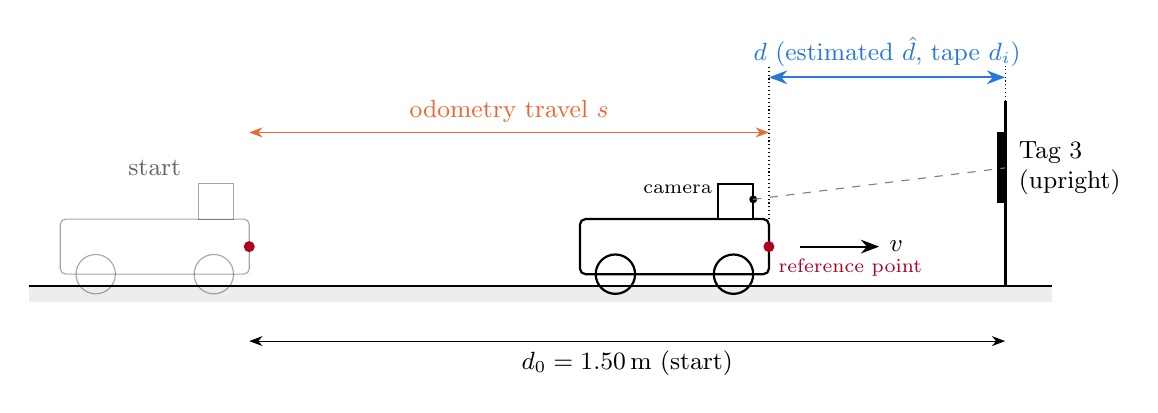
\begin{tikzpicture}[x=1.0cm,y=1.0cm,>=Stealth]
  \fill[soft] (-0.4,-0.25) rectangle (12.6,-0.05);
  \draw[thick] (-0.4,-0.05) -- (12.6,-0.05);
  % tag
  \draw[very thick] (12,-0.05) -- (12,2.3);
  \fill (11.9,1.0) rectangle (12.0,1.9);
  \node[right,align=left,font=\small] at (12.05,1.45) {Tag 3\\(upright)};
  % robot at start (faded)
  \begin{scope}[opacity=0.35]
    \draw[rounded corners=2pt,fill=white] (0,0.1) rectangle (2.4,0.8);
    \draw (0.45,0.1) circle (0.25) (1.95,0.1) circle (0.25);
    \draw[fill=white] (1.75,0.8) rectangle (2.2,1.25);
  \end{scope}
  \node[font=\small,opacity=0.6] at (1.2,1.45) {start};
  % robot at stop
  \draw[rounded corners=2pt,fill=white,thick] (6.6,0.1) rectangle (9.0,0.8);
  \draw[thick] (7.05,0.1) circle (0.25) (8.55,0.1) circle (0.25);
  \draw[fill=white,thick] (8.35,0.8) rectangle (8.8,1.25);
  \fill (8.8,1.05) circle (0.05);
  \node[font=\scriptsize,above left] at (8.4,1.0) {camera};
  \draw[dashed,gray] (8.8,1.05) -- (12,1.45);
  % reference point
  \fill[acc] (9.0,0.45) circle (0.07);
  \fill[acc] (2.4,0.45) circle (0.07);
  \node[font=\scriptsize,acc,below right] at (9.0,0.42) {reference point};
  % distances
  \draw[<->] (2.4,-0.75) -- node[below,font=\small] {$d_0=\ResStart$\,m (start)} (12,-0.75);
  \draw[<->,ckf,thick] (9.0,2.6) -- node[above,font=\small] {$d$ (estimated $\hat d$, tape $d_i$)} (12,2.6);
  \draw[densely dotted] (9.0,0.8) -- (9.0,2.75);
  \draw[densely dotted] (12,2.3) -- (12,2.75);
  \draw[<->,codo] (2.4,1.9) -- node[above,font=\small] {odometry travel $s$} (9.0,1.9);
  \draw[->,thick] (9.4,0.45) -- (10.4,0.45) node[right,font=\small] {$v$};
\end{tikzpicture}
\caption{Experiment geometry (side view, not to scale). The reference point (red) is the front face of the chassis front armour on the robot's centre line; the same point is used for the estimate and for the tape measurement. The robot starts at $d_0$ and stops when $\hat d$ reaches the stopping distance $d_{stop}$. The camera sits above and behind the reference point and looks about $20^\circ$ down; its offset is absorbed by the calibration in Eq.~\eqref{eq:calib}.}
\label{fig:setup}
\end{figure}

% =====================================================================
\section{Method}
\subsection{Software overview}
Everything runs on the laptop in one Python program (\texttt{run\_trials.py} with the package \texttt{rm\_odom\_tag}). The SDK delivers the chassis position (50\,Hz), the attitude (20\,Hz), the battery level and the H.264 video stream decoded to 1280$\times$720 images. One estimator iteration runs per camera frame; the chassis is commanded with \texttt{drive\_speed} with a 0.5\,s watchdog, so the robot stops by itself if the laptop stops sending.

\begin{center}\small
\begin{tabular}{@{}p{3.0cm}>{\raggedright\arraybackslash}p{12.8cm}@{}}
\toprule
\textbf{File} & \textbf{Purpose}\\\midrule
\texttt{kf.py} & 1-D Kalman filter (Eqs.~\ref{eq:pred}--\ref{eq:gate}), odometry history and latency compensation (Eq.~\ref{eq:lat})\\
\texttt{tag.py} & AprilTag detection, pose by \texttt{solvePnP}, plane distance (Eq.~\ref{eq:plane}), calibrated camera model (Eqs.~\ref{eq:calib}, \ref{eq:R})\\
\texttt{control.py} & speed law, steering law and stop rule (Eqs.~\ref{eq:v}--\ref{eq:stop})\\
\texttt{trial.py} & one trial: DETECT $\to$ APPROACH $\to$ SETTLE; logs every iteration, records an annotated on-board video\\
\texttt{robot\_io.py} & \texttt{SdkIO} (real robot) and \texttt{SimIO} (test simulator with the same interface)\\
\texttt{run\_trials.py} & session driver: \texttt{check}, \texttt{calib}, \texttt{warmup}, \texttt{trials}, \texttt{tape}, \texttt{sim}\\
\texttt{scripts/} & \texttt{fit\_calib.py}, \texttt{estimate\_latency.py}, \texttt{analyze.py} (errors, statistics, plots, tables)\\
\bottomrule
\end{tabular}
\end{center}

\subsection{Tag detection and the camera measurement}
Each frame is converted to grey and searched with OpenCV's \texttt{aruco} module using the AprilTag \texttt{36h11} dictionary and sub-pixel corner refinement (about 13\,ms per 720p frame on the laptop; a slower AprilTag quad detector is used only when the fast path misses the tag). Only ID~3 is accepted. With the four corner pixels $\bm u_j$ and the known corner coordinates of a square of side $\ell=0.15$\,m, the perspective-$n$-point problem
\begin{equation}
(\bm R_{ct},\bm t_{ct})=\arg\min_{\bm R,\bm t}\sum_{j=1}^{4}\left\|\bm u_j-\pi\!\left(\bm K(\bm R\,\bm X_j+\bm t)\right)\right\|^2,\qquad
\bm K=\begin{bmatrix}f_x&0&c_x\\0&f_y&c_y\\0&0&1\end{bmatrix}
\label{eq:pnp}
\end{equation}
is solved with the planar-square solver \texttt{SOLVEPNP\_IPPE\_SQUARE} ($\pi$ is the perspective division). $\bm t_{ct}$ is the tag centre and $\bm n=\bm R_{ct}\bm e_3$ the tag normal in the camera frame. The quantity used is the perpendicular distance from the camera to the tag plane,
\begin{equation}
z_{plane}=\left|\bm n^{\!\top}\bm t_{ct}\right|.
\label{eq:plane}
\end{equation}
Unlike the range $\|\bm t_{ct}\|$ or the depth $t_z$, it does not depend on the camera pitch (the EP camera looks about $20^\circ$ down) or on how high the tag is mounted, and for a robot facing the tag it equals the forward distance. The horizontal bearing $\beta=\operatorname{atan2}(t_x,t_z)$ is used for steering.

\textbf{Calibration.} The intrinsics are nominal values for the 720p stream ($f_x=634.1$, $f_y=632.5$, $c_x=634.5$, $c_y=365.2$ px), and the camera is not at the reference point. Both effects are removed by a linear model fitted, before the trials, to the robot at rest at \CalN{} tape-measured distances between 0.5 and 1.5\,m:
\begin{equation}
z=a\,z_{plane}+b,\qquad (a,b)=\arg\min\sum_{m}\big(d_m-a\,z_{plane,m}-b\big)^2 .
\label{eq:calib}
\end{equation}
$a$ absorbs focal-length and tag-size errors, $b$ the horizontal offset between camera and reference point. The frame-to-frame standard deviation at each calibration distance gives the measurement noise model
\begin{equation}
\sigma_z(z)=c_0+c_1 z^2,
\label{eq:R}
\end{equation}
because a fixed corner-pixel noise produces a distance error that grows with $z^2$ ($\partial z/\partial w=-z^2/(f\ell)$ for a tag of image width $w=f\ell/z$).

\subsection{Prediction from odometry}
The chassis position is subscribed at the start of every trial in the SDK's relative mode, which subtracts the start position but keeps the axes of the power-on frame. Because the robot only drives forward along a straight line, the forward travel is the length of the displacement, $s_k=\sqrt{x_k^2+y_k^2}$. Between two iterations the robot moved $\Delta s_k=s_k-s_{k-1}$ closer to the tag:
\begin{align}
\hat d_{k|k-1}&=\hat d_{k-1|k-1}-\Delta s_k, \label{eq:pred}\\
P_{k|k-1}&=P_{k-1|k-1}+Q_k,\qquad Q_k=(\alpha\,\Delta s_k)^2+(\sigma_v\,\Delta t_k)^2, \label{eq:Q}
\end{align}
with $\alpha=0.03$ (3\,\% odometry scale uncertainty: slip and wheel radius) and $\sigma_v=0.005$\,m/s (unmodelled motion). The filter starts at the known start distance, $\hat d_0=d_0$, with $\sigma_0=1$\,cm for placing the robot by hand. Without correction, Eq.~\eqref{eq:pred} reduces to the \emph{odometry-only} estimate $\hat d^{\,odo}_k=d_0-s_k$, whose variance grows without bound.

\subsection{Correction with the camera}
A frame received at time $t$ shows the scene at $t-L$. In the meantime the robot moved $s(t)-s(t-L)$, which is read from a buffer of time-stamped odometry, so the measurement is moved to the present before it is used:
\begin{equation}
z_k=\big(a\,z_{plane}+b\big)-\big[s(t_k)-s(t_k-L)\big].
\label{eq:lat}
\end{equation}
At 0.2\,m/s and $L\approx0.15$\,s this term is about 3\,cm, so without it the correction would pull the estimate away from the truth during the motion. The remaining timing uncertainty $\sigma_L=0.03$\,s is added to the measurement variance. The scalar Kalman correction is then
\begin{align}
y_k&=z_k-\hat d_{k|k-1}, & S_k&=P_{k|k-1}+R_k, & R_k&=\sigma_z(z_k)^2+(\sigma_L\,v_k)^2,\label{eq:innov}\\
K_k&=\frac{P_{k|k-1}}{S_k}, & \hat d_{k|k}&=\hat d_{k|k-1}+K_k\,y_k, & P_{k|k}&=(1-K_k)\,P_{k|k-1}.\label{eq:update}
\end{align}
A measurement is rejected (not used, counted) when
\begin{equation}
|y_k|>3\sqrt{S_k},
\label{eq:gate}
\end{equation}
which protects the estimate from a wrong pose (for example a flipped IPPE solution or a motion-blurred corner).
The gain $K_k\in[0,1]$ is the error-correction weight: when the prediction is uncertain ($P$ large, after travel) or the camera is precise (close to the tag), $K\to1$ and the camera dominates; when the camera is noisy (far, moving) $K$ is small and odometry dominates. Between frames in which the tag is not found, the prediction alone carries the estimate.

\subsection{Straight-line motion, speed and stop}\label{sec:steer}
\begin{align}
v_k&=\operatorname{sat}_{[v_{min},\,v_{max}]}\!\big(k_v(\hat d_k-d_{stop})\big),\quad |v_k-v_{k-1}|\le a_{max}\Delta t_k, \label{eq:v}\\
\omega_k&=\operatorname{sat}_{\omega_{max}}\!\big(k_\beta\,\beta_k\big)\quad(\text{SDK sign: } \omega>0 \text{ turns clockwise, } \beta>0 \text{ tag on the right}), \label{eq:w}\\
\text{stop when }&\ \hat d_k-d_{stop}\le v_k\,t_{lead}. \label{eq:stop}
\end{align}
with $v_{max}=0.20$\,m/s, $v_{min}=0.04$\,m/s, $k_v=0.8$\,s$^{-1}$, $a_{max}=0.25$\,m/s$^2$, $k_\beta=1.2$\,s$^{-1}$, $\omega_{max}=15^\circ$/s, $t_{lead}=0.1$\,s. There is no sideways command ($v_y=0$): the robot only drives forward and turns slightly to keep the tag centred, so the path stays on the line from the start point to the tag. Straightness is checked from the logged odometry path: its largest distance from the straight start--end line was \ResLateral\,mm on average (largest \ResLateralMax\,mm), and the tag bearing never exceeded \ResBearingMax$^\circ$ during the approaches. The slow-down near the stop (Eq.~\ref{eq:v}) keeps the braking roll-out short; the roll-out is still measured by odometry and enters the estimate through Eq.~\eqref{eq:pred}.

\subsection{Trial sequence}
\begin{center}
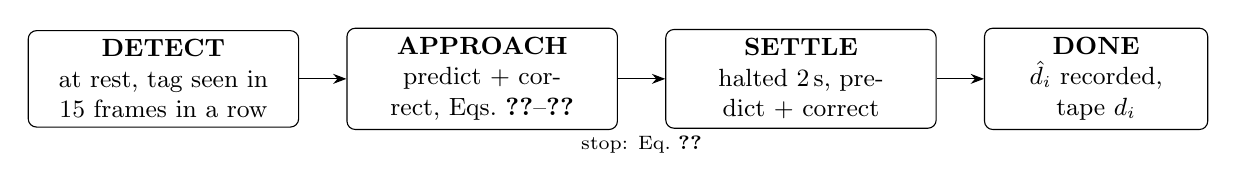
\begin{tikzpicture}[node distance=1.0cm,>=Stealth,box/.style={draw,rounded corners=3pt,align=center,font=\small,minimum height=1.1cm,text width=3.2cm}]
\node[box] (a) {\textbf{DETECT}\\at rest, tag seen in 15 frames in a row};
\node[box,right=0.6cm of a] (b) {\textbf{APPROACH}\\predict + correct, Eqs.~\ref{eq:v}--\ref{eq:w}};
\node[box,right=0.6cm of b] (c) {\textbf{SETTLE}\\halted 2\,s, predict + correct};
\node[box,right=0.6cm of c,text width=2.6cm] (d) {\textbf{DONE}\\$\hat d_i$ recorded, tape $d_i$};
\draw[->] (a) -- (b); \draw[->] (b) -- node[below=0.6cm,font=\scriptsize]{stop: Eq.~\ref{eq:stop}} (c); \draw[->] (c) -- (d);
\end{tikzpicture}
\end{center}
The final estimate $\hat d_i$ of a trial is the filter value at the end of the 2\,s settle window. The program also stores, for the same trial, the odometry-only estimate $d_0-s$ and the camera-only estimate (median of the calibrated camera distances while the robot is at rest after the stop), so the role of prediction and correction can be compared on identical runs. Safety limits stop the robot if the odometry travel exceeds $d_0-d_{stop}+0.15$\,m or the estimate falls below 0.30\,m.

\subsection{Sensor measurements used}
\begin{center}\small
\begin{tabular}{@{}>{\raggedright\arraybackslash}p{3.3cm}>{\raggedright\arraybackslash}p{3.6cm}>{\raggedright\arraybackslash}p{2.2cm}>{\raggedright\arraybackslash}p{6.0cm}@{}}
\toprule
\textbf{Measurement} & \textbf{Source} & \textbf{Rate} & \textbf{Used for}\\\midrule
Forward travel $s$ & chassis position (wheel encoders) & 50\,Hz & prediction (Eqs.~\ref{eq:pred}, \ref{eq:Q}), latency shift (Eq.~\ref{eq:lat}), safety limit\\
Tag plane distance $z_{plane}$ & camera + PnP & about 30\,Hz & \textbf{correction} (Eqs.~\ref{eq:lat}--\ref{eq:gate})\\
Tag bearing $\beta$ & camera + PnP & with each frame & steering (Eq.~\ref{eq:w})\\
Yaw, chassis $x$--$y$ position & IMU attitude, chassis position & 20 / 50\,Hz & logged; path straightness (largest distance of the path from the start--end line)\\
Tape distance $d_i$ & tape measure & once per trial & ground truth for the error (not used by the robot)\\
\bottomrule
\end{tabular}
\end{center}

% =====================================================================
\section{Experimental setup and procedure}
\begin{itemize}
\item \textbf{Robot and link:} RoboMaster EP Core, USB cable (RNDIS, robot at 192.168.42.2), Ubuntu~24.04, \texttt{robomaster} SDK, video 720p.
\item \textbf{Tag:} the same printed Tag~3 sheet as in Assignment~2 (\texttt{Assets/Tag3\_A4\_print.pdf}, \texttt{tag36h11} ID 3, black square 150\,mm; the PDF rendered back and decoded by the detector of this project gives ID 3 and 150.1\,mm), fixed upright with its centre about 10\,cm below the camera lens, perpendicular to the floor line along which the robot drives.
\item \textbf{Start distance:} $d_0=\ResStart$\,m from the tag plane to the reference point, marked on the floor with tape; the robot is placed on the mark, facing the tag, in every trial.
\item \textbf{Stopping distance:} $d_{stop}=\ResStop$\,m, the same in every trial; the robot stops well before the tag.
\item \textbf{Reference point:} the front face of the chassis front armour on the centre line, for the estimate (through the calibration) and for the tape measurement.
\item \textbf{Floor and light:} carpet floor in a dorm room, indoor ceiling lights.
\end{itemize}
Procedure: (1) \texttt{run\_trials.py check}: link, battery, camera and tag detection at rest; (2) \texttt{calib}: robot at rest at five tape-measured distances, 60 frames each, then Eq.~\eqref{eq:calib} is fitted; (3) \texttt{warmup}: two full runs that are \emph{not} part of the results, used to estimate the latency $L$ (Section~\ref{sec:lat}); (4) \texttt{trials}: ten trials. After each trial the robot is left exactly where it stopped, the distance from the tag plane to the reference point is measured with a steel tape (resolution 1\,mm) along the floor, and the value is typed into the program, which writes it next to the estimates in \texttt{logs/trials.csv}. The estimate is printed before the tape is read, but it is not used to take the measurement. Four earlier runs are not in the results and are kept in \texttt{logs/trials\_invalid/}: in three of them the tag stand had shifted, so the tape was read from a zero line no longer under the tag (the camera saw the robot stop at the same place, within 4\,mm, while the tape readings fell from 47 to 40\,cm); in the fourth the robot was not on the start mark and drove into the stand. A start-position check (camera within 10\,cm of $d_0$, otherwise the robot does not move) was added after that run.

\subsection{Camera calibration result}
\begin{center}\small
\tabortodo{tab_calib.tex}{calibration table (run \texttt{calib})}

\vspace{6pt}
\figorti{../figures/fig_calib.png}{0.85}{calibration figure}
\end{center}
Fit: $a=\CalA$, $b=\CalB$\,m, residual RMS \CalRMS\,mm; noise model $\sigma_z=\CalCzero\,\text{mm}+\CalCone\,\text{mm/m}^2\,z^2$.

\subsection{Camera latency}\label{sec:lat}
In the warm-up runs the calibrated camera distance $z(t)$ is compared with the odometry trajectory shifted by a trial latency, $c-s(t-L)$, over all frames with $v>0.05$\,m/s; $c$ is fitted per run and $L$ is chosen on a 5\,ms grid to minimise the RMS residual. From \LatRuns{} warm-up runs: $L=\LatL$\,s, residual RMS \LatRMS\,mm (\LatRMSzero\,mm with no compensation).
\begin{center}\figorti{../figures/fig_latency.png}{0.48}{latency figure (run \texttt{warmup})}\end{center}

% =====================================================================
\section{Error calculation and statistical analysis}
For trial $i$ the final distance estimation error (estimate minus tape) is
\begin{equation}
e_i=\hat d_i-d_i,\qquad i=1,\dots,n,
\label{eq:err}
\end{equation}
so $e_i>0$ means the robot believed it was further from the tag than it really was. Over the $n$ trials:
\begin{align}
\text{bias } \bar e&=\frac1n\sum_{i=1}^n e_i, & s&=\sqrt{\frac{1}{n-1}\sum_{i=1}^n (e_i-\bar e)^2},\\
\text{MAE}&=\frac1n\sum_{i=1}^n |e_i|, & \text{RMSE}&=\sqrt{\frac1n\sum_{i=1}^n e_i^2}=\sqrt{\bar e^{\,2}+\tfrac{n-1}{n}s^2},\\
\text{range}&=\max_i e_i-\min_i e_i, & \text{95\,\% CI}&=\bar e\pm t_{0.975,\,n-1}\frac{s}{\sqrt n}.
\end{align}
The MAE and the range are the two quantities asked for in the brief. The bias tells whether the method has a systematic error (tested with a one-sample $t$-test, $t=\bar e\sqrt n/s$, $H_0{:}\ \mu_e=0$); $s$ and the range describe the consistency of the trials. A Shapiro--Wilk test checks whether the errors are compatible with a normal distribution (needed for the $t$-based interval). The paired Wilcoxon signed-rank test compares $|e_i|$ of the fused estimate with $|e_i|$ of odometry only and camera only on the same trials, without assuming normality. Finally, the filter's own uncertainty is checked: if $\sigma_{KF}$ is realistic, about 95\,\% of the errors should satisfy $|e_i|\le2\sigma_{KF,i}$.

The same error is computed for the two single-sensor estimates of every trial, $e^{odo}_i=(d_0-s_i)-d_i$ and $e^{cam}_i=\hat d^{\,cam}_i-d_i$. The correction applied by the camera in trial $i$ is $\hat d_i-\hat d^{\,odo}_i$.

% =====================================================================
\section{Results}
\subsection{Trial table}
\begin{table}[H]\centering\small
\caption{Final distance per trial. $\hat d_i$: estimate, $d_i$: tape measurement (same reference point), $e_i=\hat d_i-d_i$. $\sigma_{KF}$: filter standard deviation at the end of the trial.}
\label{tab:trials}
\tabortodo{tab_trials.tex}{trial table (written by \texttt{scripts/analyze.py} after the trials)}
\end{table}

\subsection{Statistics}
\begin{table}[H]\centering\small
\caption{Error statistics over the \ResN{} trials (Eq.~\ref{eq:err}; positive = estimate further than the tape).}
\label{tab:stats}
\tabortodo{tab_stats.tex}{statistics table}
\end{table}
\IfFileExists{../figures/term_analyze.png}{\begin{center}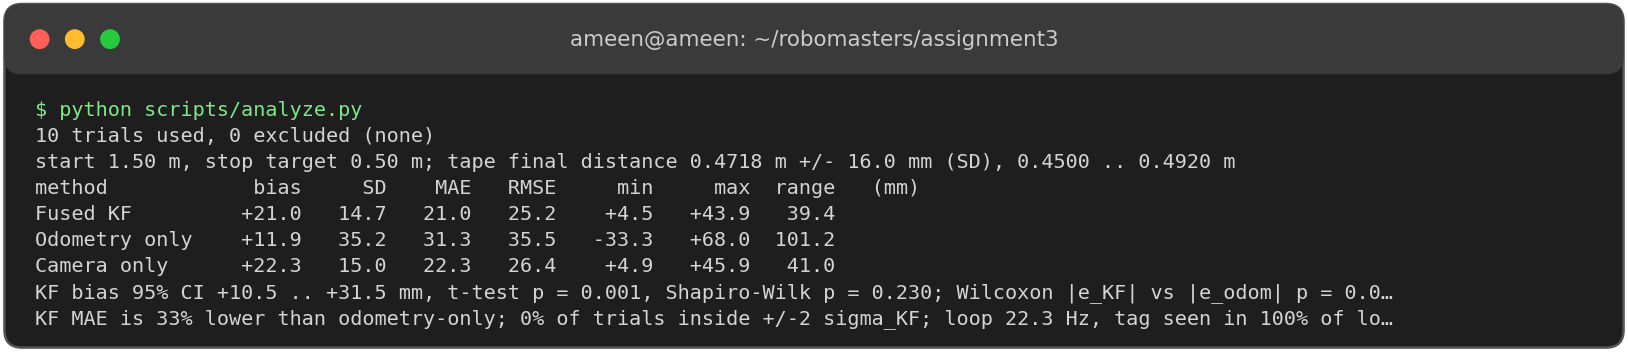
\includegraphics[width=0.95\linewidth]{../figures/term_analyze.png}\end{center}}{}
Fused estimate: \textbf{MAE \ResMAE\,mm}, \textbf{range of errors \ResRange\,mm} (from \ResMin{} to \ResMax\,mm), bias \ResBias\,mm (95\,\% CI \ResCI\,mm, $t$-test $p=\ResPt$), SD \ResSD\,mm, RMSE \ResRMSE\,mm. Shapiro--Wilk $p=\ResPsw$. \ResCover\,\% of the trials lie within $\pm2\sigma_{KF}$ (mean $\sigma_{KF}$ \ResSigmaMean\,mm).

\subsection{Scatter plot of each trial}
Figure~\ref{fig:grid} shows the last 3\,s of every trial (stop and settle), where the final estimate is formed: each camera measurement $z_k$ is a point, the odometry-only estimate is the dashed line, the fused estimate is the solid line with its $\pm2\sigma$ band, and the star is the tape measurement. The full run of every trial (start to stop) is in Appendix~\ref{app:trials}.
\begin{figure}[H]\centering
\figorti{../figures/fig_trials_grid.png}{0.92}{per-trial scatter grid (after the trials)}
\caption{Per-trial scatter plots, last 3\,s of each trial. The vertical line marks the stop command.}
\label{fig:grid}
\end{figure}

\subsection{Final scatter plot}
\begin{figure}[H]\centering
\figorti{../figures/fig_final_scatter.png}{1.0}{final scatter plot (after the trials)}
\caption{Left: estimated against measured final distance for all trials and the three estimators; points on the diagonal have zero error. Right: error of every trial with the bias and the $\pm2$\,SD band of the fused estimate.}
\label{fig:final}
\end{figure}
\begin{figure}[H]\centering
\figorti{../figures/fig_error_box.png}{0.72}{error distribution figure (after the trials)}
\caption{Distribution of the final errors (box: quartiles, line: median, points: trials).}
\label{fig:box}
\end{figure}

% =====================================================================
\section{Discussion}
\subsection{Consistency of the trials}
The robot stopped at a tape distance of \ResStopMean\,m on average, with an SD of \ResStopSD\,mm (from \ResStopMin{} to \ResStopMax\,m), so the stopping behaviour itself repeats closely. The fused estimation error has an SD of \ResSD\,mm and a range of \ResRange\,mm over \ResN{} trials, against \ResOdomSD\,mm and \ResOdomRange\,mm for odometry alone. Every one of the ten errors is positive (+4.5 to +43.9\,mm), so the scatter in Table~\ref{tab:trials} is mostly one common bias rather than random noise. The largest errors are in trials 3--5 (+30.5 to +43.9\,mm), measured while the tag stand was still being re-fixed and the start mark re-measured, while trials 8--10 stayed within +8\,mm. In the same ten trials odometry alone swung from $-33$ to $+68$\,mm because of how precisely the robot was placed on the start mark, and the camera removed that start-position error.

\subsection{Possible sources of error}
\begin{itemize}
\item \textbf{Tape measurement and reference point:} the tape is read to about 1\,mm, but holding it perpendicular to the tag plane and on the reference point adds a few mm.
\item \textbf{Camera model:} nominal intrinsics, no distortion model, and a printed tag that may not be exactly 15.0\,cm or perfectly flat; the linear calibration (Eq.~\ref{eq:calib}) removes the scale and offset part, the residual RMS (\CalRMS\,mm) is what remains. Corner noise grows with $z^2$ (Eq.~\ref{eq:R}).
\item \textbf{Camera latency:} a wrong $L$ biases the moving measurements by $v\,\Delta L$ (2\,mm per 10\,ms at 0.2\,m/s); after the stop this vanishes, which is why the final estimate is taken after the settle window.
\item \textbf{Odometry:} wheel slip at start and braking, wheel-radius and mecanum roller errors; these accumulate over the 1\,m path and explain the larger spread of the odometry-only error (bias \ResOdomBias\,mm).
\item \textbf{Placement and heading:} the robot is placed by hand on the start mark (about $\pm5$\,mm, a few degrees). A small heading error makes the plane distance and the tape line differ by a factor $\cos\psi$ ($<0.2$\,mm for $\psi=1^\circ$ at 0.5\,m).
\item \textbf{Calibration bias carried into all trials:} the same $(a,b)$ is used in every trial, so any calibration error shows up as a common bias, not as scatter; the bias and its confidence interval separate this from the random error.
\end{itemize}

\subsection{Role of prediction and correction}
\textbf{Prediction} (odometry) gives a smooth, delay-free estimate at every iteration and carries the estimate through frames without a detection and through the braking roll-out (mean \ResRollout\,cm after the stop command). On its own its error grows with the distance travelled: over the trials the odometry-only final estimate has an MAE of \ResOdomMAE\,mm and a range of \ResOdomRange\,mm.
\textbf{Correction} (camera) bounds this drift: every frame pulls the estimate towards the measured tag distance with the gain $K_k$, and the total correction applied at the end of a trial (fused minus odometry-only) averaged \ResCorrMean\,mm (largest \ResCorrMaxAbs\,mm). The fused estimate reaches an MAE of \ResMAE\,mm, \ResImprove\,\% lower than odometry alone (Wilcoxon $p=\ResWilOdom$). Compared with the camera alone (MAE \ResCamMAE\,mm, Wilcoxon $p=\ResWilCam$), the filter adds smoothness during the motion, rejects outliers through the gate, and continues when the tag is lost, which a camera-only stop rule could not do. In these data the fused estimate is limited by the camera at rest: its error follows the camera-only error within 3\,mm in every trial (bias +21.0 vs +22.3\,mm), so the remaining bias comes from the camera calibration (no calibration point below 0.75\,m, and two inconsistent 1.50\,m points), not from the filter.

% =====================================================================
\section{Verification}
\begin{itemize}
\item 16 unit and pipeline tests (\texttt{python -m pytest -q tests}) cover the Kalman equations against the closed-form scalar results, the gate, the latency buffer, the speed and steering laws (including the SDK sign of $\omega$), the plane distance from rendered tag images at 0.5, 1.0 and 1.5\,m with a yawed robot, rejection of a wrong tag ID, the calibration fit, a complete simulated trial followed by the analysis scripts, and the robot interface against a stub of the SDK (connection, 720p stream, odometry travel in the unaligned SDK frame, the 0.5\,s drive watchdog, stop on close).
\item The simulator (\texttt{SimIO}) renders the real tag from the true pose, delays frames by a latency, adds a wheel-odometry scale error, pixel noise, command delay and a first-order speed response. It was used only to test the code; none of its numbers appear in the results.
\end{itemize}
\begin{center}\figorti{../figures/term_pytest.png}{0.95}{terminal capture of the tests}\end{center}

\section{Deliverables}
\begin{itemize}
\item Report: this document.
\item Code: \url{https://github.com/AmeenUrRehman/RoboMaster-Advanced-Robotics}, folder \texttt{Assignment 3} (package, session driver, analysis scripts, tests, logs of all trials, figures, report source).
\item Video: \videolink{} (the robot detects the tag and drives to it; the on-board view with the live estimate is recorded by the program for every trial).
\end{itemize}

\appendix
\section{Full run of every trial}\label{app:trials}
Each plot shows the complete trial (left) and its stop and settle phase (right), with the camera measurements as points.
\IfFileExists{../figures/fig_trial_01.png}{%
\foreach \i in {01,02,03,04,05,06,07,08,09,10}{%
  \IfFileExists{../figures/fig_trial_\i.png}{\par\noindent\includegraphics[width=\linewidth]{../figures/fig_trial_\i.png}\par\medskip}{}}%
}{\todo{per-trial figures (after the trials)}}

\section{How to run}
\begin{Verbatim}[fontsize=\small,frame=single]
source ~/rm_setup.sh && cd "Assignment 3"
python -m pytest -q tests                 # 16 tests, no robot needed
python run_trials.py session              # all steps below, in order
python run_trials.py check                # robot link, camera, tag
python run_trials.py calib                # 5 distances at rest -> config/calib.json
python run_trials.py warmup               # 2 runs -> config/latency.json
python run_trials.py trials --n 10        # measured trials, tape typed after each
python scripts/analyze.py                 # errors, statistics, plots, LaTeX tables
\end{Verbatim}

\section{Source listing: \texttt{kf.py}}
\VerbatimInput[fontsize=\scriptsize,frame=single]{../rm_odom_tag/kf.py}

\end{document}
